% !TEX program = xelatex
\documentclass[a4paper,11pt,fontset=none]{ctexart}
\usepackage{fontspec}
\setmainfont{Times New Roman}
\setCJKmainfont{Songti SC}
\setCJKsansfont{Songti SC}
\setCJKmonofont{Songti SC}
\usepackage{geometry}
\geometry{left=2.45cm,right=2.45cm,top=2.35cm,bottom=2.35cm}
\usepackage{graphicx}
\graphicspath{{../images/}{figures/}}
\usepackage{booktabs,tabularx,array,longtable}
\usepackage[table]{xcolor}
\usepackage{enumitem,fancyhdr,titlesec,amsmath,float,caption,hyperref,url}
% 比赛提交规范：报告内所有文字统一使用纯黑色；颜色仅保留在插图图形元素中。
\definecolor{DeepBlue}{RGB}{0,0,0}
\definecolor{AcademicBlue}{RGB}{0,0,0}
\definecolor{AccentRed}{RGB}{0,0,0}
\definecolor{SoftGray}{HTML}{F3F4F6}
\hypersetup{hidelinks,pdftitle={ESASR 技术迭代与问题解决记录},pdfauthor={Justifying}}
\setlength{\parindent}{2em}
\linespread{1.18}
\renewcommand{\arraystretch}{1.18}
\setlist[itemize]{leftmargin=2em,itemsep=0.12em}
\captionsetup{font=small,labelfont=bf,labelsep=quad}
\pagestyle{fancy}
\fancyhf{}
\fancyhead[C]{\small ESASR 技术迭代与问题解决记录}
\cfoot{\small\thepage}
\renewcommand{\headrulewidth}{0.5pt}
\titleformat{\section}{\zihao{3}\bfseries\color{DeepBlue}}{\thesection}{0.8em}{}
\titleformat{\subsection}{\zihao{4}\bfseries\color{DeepBlue}}{\thesubsection}{0.7em}{}
\renewcommand{\tabularxcolumn}[1]{m{#1}}
\newcolumntype{Y}{>{\raggedright\arraybackslash}X}
\newcolumntype{C}[1]{>{\centering\arraybackslash}m{#1}}

\begin{document}
\color{black}
\pagenumbering{Roman}
\thispagestyle{empty}
\begin{center}
\vspace*{2.1cm}
{\fontsize{25pt}{34pt}\selectfont\bfseries\color{DeepBlue} ESASR\par}
\vspace{0.3cm}
{\zihao{4}\bfseries Evidence-State Adaptive Scholarly Retrieval\par}
\vspace{0.6cm}
{\zihao{1}\bfseries 技术迭代与问题解决记录\par}
\vspace{0.7cm}
{\zihao{3}第八届中国研究生人工智能创新大赛附加材料\par}
\vfill
{\zihao{4}\bfseries 团队名称：Justifying\par}
\vspace{0.25cm}
{\zihao{4}\bfseries 提交日期：2026年8月31日\par}
\vspace{1cm}
\end{center}

\newpage
{\small\tableofcontents}
\newpage
\pagenumbering{arabic}

\section{文档定位与阅读方式}

本材料是项目主报告的过程审计层，集中记录架构探索、模块替换、参数选择、对照结论、工程改进与验证闭环。主报告只叙述最终提交方案“证据状态驱动的自适应学术检索框架（ESASR）”；本材料保留从早期原型到最终方案的完整技术债务和证据链。两份文档的分工如下：

\begin{table}[H]
\centering
\caption{主报告与附加材料的内容边界}
\begin{tabularx}{\textwidth}{C{3cm} Y Y}
\toprule
\textbf{材料} & \textbf{回答的问题} & \textbf{内容} \\
\midrule
项目主报告 & 最终方案是什么、为何合理、证据有多强 & 单一方法主线、核心实验、系统完成度、应用与边界 \\
本附加材料 & 如何收敛到最终方案、如何识别改进空间、如何复现 & 迭代时间线、详细消融、对照结论、改进闭环、参数与归档位置 \\
\bottomrule
\end{tabularx}
\end{table}

为避免事后合理化，本记录坚持三条原则：第一，正向结果与对照结论同时保留；第二，代码实现、实验验证和强效果结论分级标记；第三，任何未在冻结协议下验证的机制均列为待验证，不因其架构完整而推断质量收益。

\section{技术演进总览}

\begin{figure}[H]
\centering
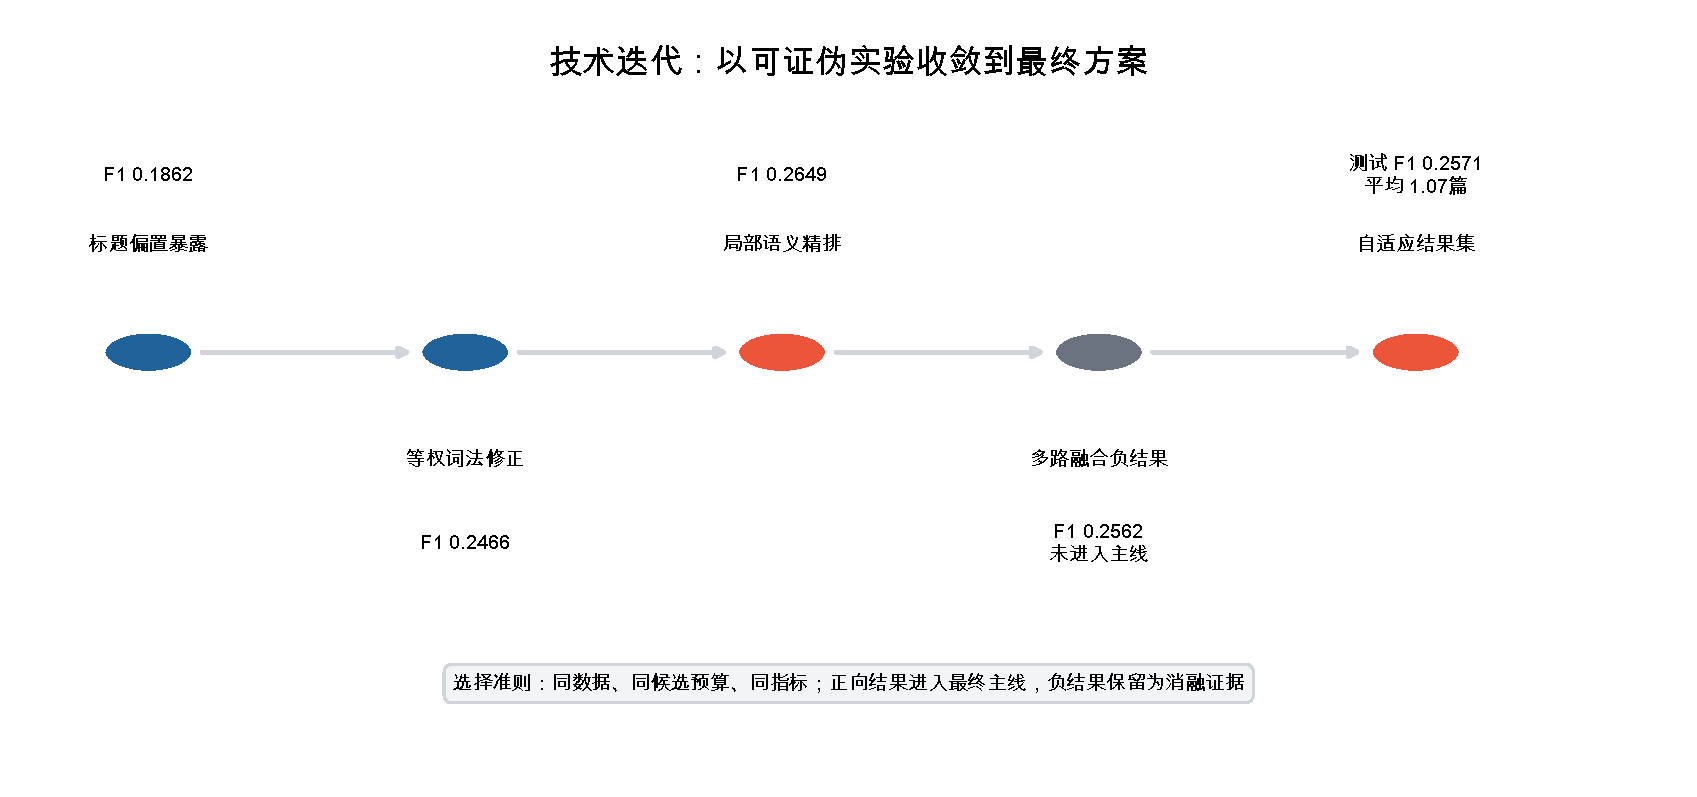
\includegraphics[width=\textwidth]{Fig10_Iteration_Roadmap.pdf}
\caption{以可证伪实验收敛最终方案。标题权重、语义精排、RRF 路由和自适应输出均在相同数据或冻结候选条件下比较；未带来收益的方案不进入最终主线。}
\label{fig:roadmap}
\end{figure}

\begin{longtable}{C{1.4cm} C{2.4cm} >{\raggedright\arraybackslash}m{4.6cm} >{\raggedright\arraybackslash}m{5.8cm}}
\caption{项目与文档演进记录}\label{tab:history}\\
\toprule
\textbf{标识} & \textbf{日期} & \textbf{主要变化} & \textbf{形成的可审计产物} \\
\midrule
\endfirsthead
\toprule
\textbf{标识} & \textbf{日期} & \textbf{主要变化} & \textbf{形成的可审计产物} \\
\midrule
\endhead
v0.1 & 2026.05.22 & 完成赛题拆解、用户需求与验收口径定义 & 需求清单、范围边界与项目文档基线 \\
v0.2 & 2026.06.12 & 完成总体架构、数据流和外部接口设计 & 架构图、接口规范与研发计划 \\
v0.3 & 2026.07.10 & 完成查询编译、缺口路由、多源检索与排序链路 & 可运行端到端原型、模块接口与测试样例 \\
v0.4 & 2026.08.08 & 冻结数据划分、基线、消融和输出策略评测协议 & 实验脚本、候选集、指标、区间与错误分析 \\
v0.5 & 2026.08.26 & 完成系统集成、回归测试、故障处理和材料一致性校验 & 稳定演示系统、测试记录与候选提交材料 \\
v1.0 & 2026.08.31 & 完成版本冻结、复现入口复核和最终提交定版 & 最终报告、附加材料、代码仓库与演示资产 \\
\bottomrule
\end{longtable}

\section{检索排序方案的收敛过程}

\subsection{V1：标题偏置词法召回}

早期本地检索使用 SQLite FTS5，标题权重 5、摘要权重 1。其动机是题名通常浓缩论文主题，但该设置放大了查询词表面重合，导致“标题像答案、摘要语义不匹配”的候选占据首位。在固定 200 条样本上，P@1 为 0.2250、R@1 为 0.1745、Macro F1@1 仅 0.1862。问题定位并非召回数量不足，而是标题信号压倒摘要证据。

\subsection{V2：标题与摘要等权}

将标题和摘要权重均设为 1 后，P@1 提升至 0.3000，Macro F1@1 提升至 0.2466，绝对增量 0.0604。该结果说明最有效的早期改动不是引入复杂网络，而是纠正已有特征的权重失衡。这一事实被保留在主报告消融中，用于防止把所有收益归因于 Cross Encoder。

\subsection{V3：局部 Cross Encoder 精排}

在相同 Top-100 候选池内，本地 \texttt{cross-encoder/ms-marco-MiniLM-L6-v2} 仅重排 Top-20，并按 0.65 语义分数与 0.35 基础分数融合。Macro F1@1 达到 0.2649，较 V2 增加 0.0183；平均端到端延时 741.7\,ms，平均精排耗时 285.3\,ms。配对差值区间跨越 0，因此该模块被判断为“方向合理、工程可用、统计证据仍不足”。

\subsection{多路 RRF 融合的对照分析}

多路检索和 RRF 的理论预期是提高不同表达的覆盖，但在相同 200 条样本上 F1@1 为 0.2562，低于 单路局部精排方案的 0.2649，平均延时也升至 905.0\,ms。可能原因包括：本地语料上的各路词法结果高度相关，RRF 增加的不是互补证据而是重复噪声；融合顺序改变了 Cross Encoder 候选池；当前查询样本对路由多样性的需求不足。该结果清晰界定了多路融合的适用条件，并为最终采用更高效的候选组织方式提供了直接实验依据。

\subsection{V5：自适应结果集}

固定 Top-1 在多答案查询上可能丢失相关论文，但固定扩大 $K$ 又迅速增加误报。为隔离“检索排序”与“输出数量”的影响，V5 直接读取冻结候选，不重新召回或精排。200 条查询按来源拆为 100 条开发集和 100 条测试集；开发集搜索 8,064 组阈值组合，测试集只使用最终规则。CARS 测试 F1 为 0.2571，固定 Top-1 为 0.2475，平均仅多返回 0.07 篇。由于配对区间包含 0，最终报告将其写为小幅正向趋势。

\begin{figure}[H]
\centering
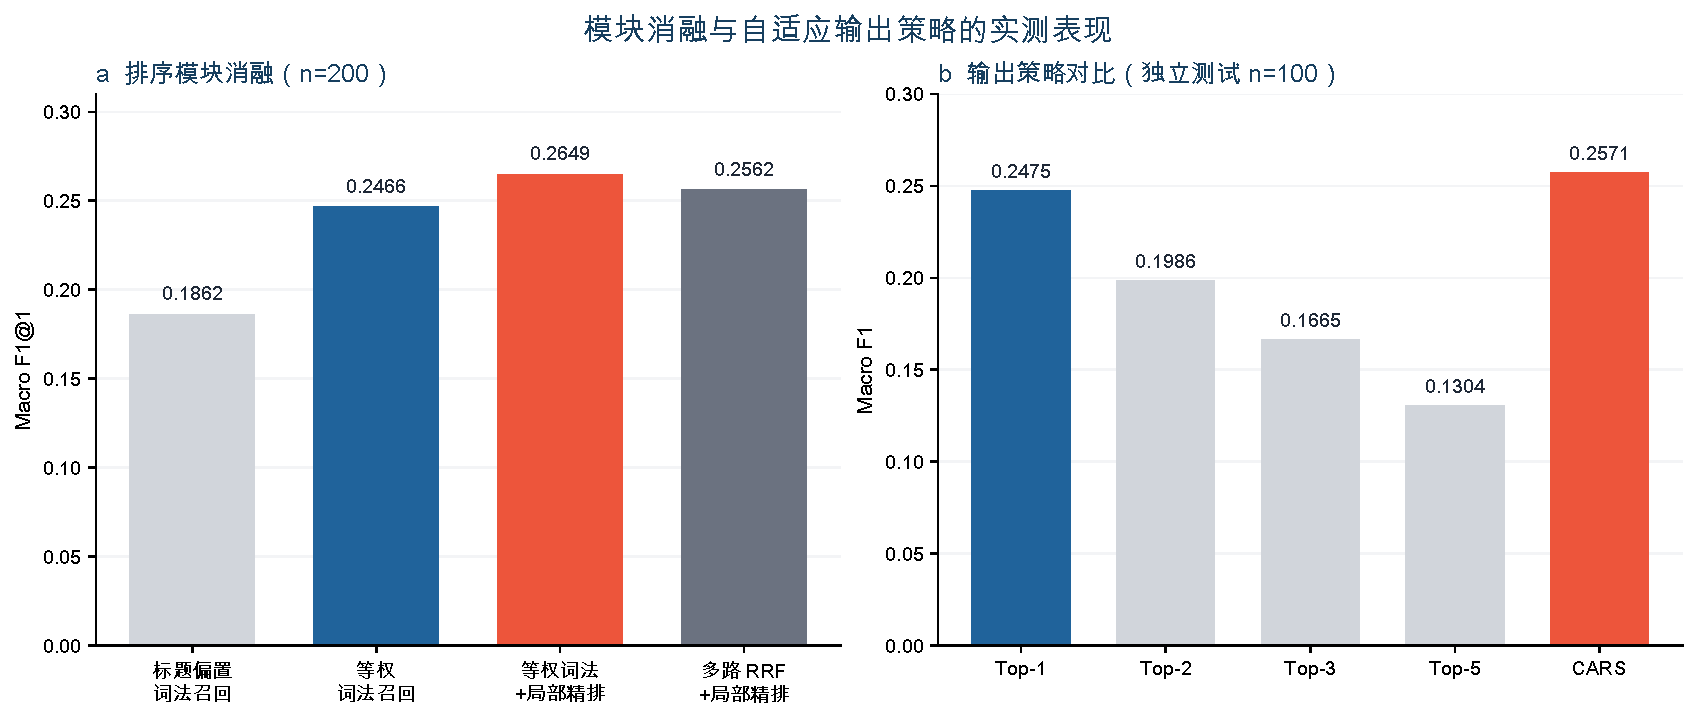
\includegraphics[width=\textwidth]{Fig8_Ablation_Performance.pdf}
\caption{各中间方案的量化比较。左图记录排序方案收敛，右图记录固定 Top-K 与 CARS 的输出策略对照。}
\label{fig:ablation}
\end{figure}

\begin{table}[H]
\centering
\caption{V1--V4 固定样本比较（$n=200$）}
\small
\begin{tabular}{C{2.1cm} C{4.0cm} C{1.25cm} C{1.25cm} C{1.25cm} C{2.5cm}}
\toprule
\textbf{方案} & \textbf{关键配置} & \textbf{P@1} & \textbf{R@1} & \textbf{F1@1} & \textbf{F1 95\% CI} \\
\midrule
V1 & 标题 5、摘要 1 & 0.2250 & 0.1745 & 0.1862 & [0.1377, 0.2371] \\
V2 & 标题 1、摘要 1 & 0.3000 & 0.2301 & 0.2466 & [0.1928, 0.3015] \\
V3 & V2 + CE Top-20 & 0.3300 & 0.2454 & 0.2649 & [0.2092, 0.3226] \\
V4 & 多路 RRF + CE Top-20 & 0.3200 & 0.2389 & 0.2562 & [0.1982, 0.3132] \\
\bottomrule
\end{tabular}
\end{table}

\begin{table}[H]
\centering
\caption{V5 独立测试集详细对照（$n=100$）}
\small
\begin{tabular}{C{2.2cm} C{1.3cm} C{1.3cm} C{1.5cm} C{2.4cm} C{1.8cm}}
\toprule
\textbf{策略} & \textbf{P} & \textbf{R} & \textbf{F1} & \textbf{F1 95\% CI} & \textbf{平均返回数} \\
\midrule
Top-1 & 0.3300 & 0.2241 & 0.2475 & [0.1715, 0.3255] & 1.00 \\
Top-2 & 0.1900 & 0.2537 & 0.1986 & [0.1424, 0.2537] & 2.00 \\
Top-3 & 0.1400 & 0.2697 & 0.1665 & [0.1219, 0.2105] & 3.00 \\
Top-5 & 0.0960 & 0.2926 & 0.1304 & [0.0991, 0.1627] & 5.00 \\
CARS & 0.3350 & 0.2374 & 0.2571 & [0.1812, 0.3350] & 1.07 \\
\bottomrule
\end{tabular}
\end{table}

\section{技术瓶颈与问题解决闭环}

\begin{longtable}{C{1.0cm} C{3.0cm} >{\raggedright\arraybackslash}m{3.85cm} >{\raggedright\arraybackslash}m{4.45cm} C{1.6cm}}
\caption{核心技术问题、定位、修复与验证}\label{tab:issues}\\
\toprule
\textbf{编号} & \textbf{改进目标} & \textbf{原因分析} & \textbf{解决方案与验证} & \textbf{状态} \\
\midrule
\endfirsthead
\toprule
\textbf{编号} & \textbf{改进目标} & \textbf{原因分析} & \textbf{解决方案与验证} & \textbf{状态} \\
\midrule
\endhead
P01 & 标题相似但任务不相关的论文居首 & 标题权重过高，摘要证据被压制 & 标题摘要等权；F1 从 0.1862 升至 0.2466 & 已闭环 \\
P02 & 词法召回无法识别语义等价表达 & 仅依赖词项匹配 & Top-20 本地 Cross Encoder；真实案例将 LoFTR 提升至首位 & 已闭环 \\
P03 & 识别多路融合的适用条件 & 各路候选高度相关并带入重复噪声 & 保留对照结果，默认不采用该路由；后续开展跨域验证 & 对照结论 \\
P04 & 优化固定 Top-K 的误报问题 & 多答案召回收益小于误报损失 & CARS 仅在三门同时满足时增加第二篇 & 已验证趋势 \\
P05 & 缺失年份/摘要/DOI 被默认值掩盖 & 展示逻辑把“未知”当成“有值” & 保持 null，增加 \texttt{metadataMissing} 并回归测试 & 已闭环 \\
P06 & 外部失败时演示论文可能污染真实结果 & 严格检索与兼容展示边界不清 & 完整检索传播失败；离线卡片统一来源标识 & 已闭环 \\
P07 & related works 被误画为引用边 & 不同关系共享一个边类型 & 分离有向 \texttt{CITES} 与无向 \texttt{RELATED} & 已闭环 \\
P08 & 保证无模型平台 Key 时仍可检索 & 规划与远端模型强绑定 & 增加确定性规则规划器与统一输出模式 & 已闭环 \\
P09 & 健康端点可达但依赖已失效 & 只检查 HTTP 可达性 & 聚合组件状态，异常返回 503/degraded & 已闭环 \\
P10 & 导出链接可能指向错误页面 & DOI、来源 URL 与 PDF URL 混用 & 按 DOI/来源映射，PDF 仅使用有效 OA 地址 & 已闭环 \\
P11 & 进一步降低前端首包体积 & Element Plus、ECharts、G6 同步打包 & 已确认构建可用；按需引入与拆包已纳入计划 & 已规划 \\
P12 & 扩展在线补检增益证据 & 本地静态语料不包含真实 API 漂移与引文图 & 已设计冻结响应、等预算三组对照协议 & 协议已设计 \\
\bottomrule
\end{longtable}

\section{关键参数与选择依据}

\begin{table}[H]
\centering
\caption{最终提交配置及证据依据}
\begin{tabularx}{\textwidth}{C{3.2cm} C{2.4cm} Y}
\toprule
\textbf{参数} & \textbf{取值} & \textbf{依据与边界} \\
\midrule
词法标题/摘要权重 & 1/1 & 固定 200 条样本显著优于 5/1；仍需跨语料敏感性分析 \\
候选池 & Top-100 & 保留排序诊断与可复现候选；不是最终输出规模 \\
Cross Encoder 范围 & Top-20 & 在当前 CPU 环境兼顾语义收益与 285.3\,ms 平均推理耗时 \\
最终融合权重 & 0.65/0.35 & 当前实验配置；未宣称理论最优 \\
子查询上限 & 4 & 控制计划扩张；两来源对应最多 8 个逻辑任务 \\
CARS 最大输出 & 2 & 开发集搜索后选定，避免固定扩展造成误报 \\
CARS 三门阈值 & 0.60/0.85/0.10 & 仅由 100 条开发集选择，测试集不参与调参 \\
bootstrap 次数 & 主评测 1,000；配对 5,000 & 用于区间估计；样本不足仍会导致宽区间 \\
\bottomrule
\end{tabularx}
\end{table}

\section{复现实验与资产索引}

排序实验归档于 \texttt{esasr-api/evaluation/experiments/} 下的 ScholarGym 离线目录，包含 Gold、逐查询预测、指标、排行榜、比较报告和 manifest。自适应选择目录包含开发/测试 Gold、固定 $K$ 预测、CARS 预测、阈值搜索与配对结果。复现时应先记录代码提交、Python/Node 依赖、模型名称与 revision、随机种子、数据文件哈希和配置哈希，再运行评测脚本；不得只保留汇总表而丢失逐查询记录。

建议的验收顺序为：运行后端 63 项与 CLI 9 项测试；执行前端生产构建；复跑排序实验并核对 F1@1=0.2649、平均时延 741.7\,ms；复跑一至两篇的受控自适应输出实验并核对 CARS F1=0.2571、平均返回数 1.07；使用 DeepSeek-V4-Flash-0731 绕过规划缓存复跑 30 条在线样本，并核对 API \texttt{usage} 总 Token 为 24,840；再验证五档置信质量动态截断的近似并列保留、80\%质量覆盖和广泛档相关性边界；启动容器服务并检查 503/degraded 语义；模拟无模型平台 Key、精排不可用和学术 API 异常；最后核对来源、缺失字段和关系分型。

所有新绘学术图片均位于项目根目录 \texttt{/images}，使用“图序号\_方法名\_用途”命名，并同时保留 PNG、SVG 与 PDF。PNG 用于主报告稳定编译，SVG 用于后续编辑，PDF 用于字形与矢量质量审计。

\section{扩展验证计划与实验契约}

\begin{enumerate}
  \item \textbf{在线 EGRR 效果：}冻结 API 响应，设置无补检、固定二轮、缺口驱动三组，在相同任务上限下报告 F1、覆盖率、HTTP 尝试和单位真阳性成本。
  \item \textbf{查询编译准确率：}建立按主题、方法、数据集、年份、Venue、开放获取和排除条件分层的人工标注集，报告槽位 F1 与硬约束违反率。
  \item \textbf{CARS 外部有效性：}在更大跨学科测试集上预注册当前阈值，不重新调参，报告配对区间和按 Gold 规模分组的收益。
  \item \textbf{系统压力与恢复：}在固定硬件上报告并发 1/5/20 的 p50/p95 时延、错误率、缓存命中率和依赖恢复时间。
  \item \textbf{真实应用验证：}开展跨学科高校课题组测试，记录任务完成时间、有效论文率、重复检索率、结果修正次数和来源核验行为。
\end{enumerate}

只有当相应实验完成并得到冻结证据后，机制才可从“已实现”升级为“已证实有效”。若结果为负，应继续保留原始数据和分析，而不是从提交材料中删除。

\section{审计结语}

项目最终方案不是按时间顺序累积全部尝试，而是由受控实验筛选得到：等权词法修复了明显偏置，局部精排提供语义增益，多路 RRF 经对照验证后退出默认路径，CARS 在冻结候选上以极小输出扩张取得初步正向结果。可信数据边界与故障传播则把“能运行”提升为“结果可追责”。后续将优先扩大独立测试规模，完成在线等预算消融与真实用户验证，使当前的可运行、可追责优势进一步转化为跨领域的稳定效果。

\end{document}
